%-------------------------------------------------------------------------------
% yum_new_gui
%-------------------------------------------------------------------------------
%
% \file        yum_new_gui.tex
% \library     Documents
% \author      Will Godfrey
% \date        2021-07-21
% \update      2021-10-08
% \version     $Revision$
% \license     $XPC_GPL_LICENSE$
%
%     Describes the changes in the GUI structure.
%
%-------------------------------------------------------------------------------

\section{Revised Graphical Interface}
\label{sec:revised_interface}
   When \textsl{Yoshimi} forked from \textsl{ZynAddSubFX}, all windows were
   a fixed size, which suited the resolution of monitors of that time.
   As resolution increased over the years,
   \textsl{Yoshimi's} windows became progressively smaller.
   Eventually we received complaints about this.
   It came to head with the introduction of 4K
   screens. On such a display a magnifying glass was needed to read the text!

   FLTK 1.3.x has some resize capability and will keep the graphics mostly in
   scale, but not the text, nor things like tabs and menu bars. Therefore we had
   to develop work-arounds and emulations for these. Eventually the following
   decisions were made:

   \begin{itemize}
      \item All windows will be independently re sizeable up to the full
         screen size.
      \item Windows and their contents will stay in scale.
      \item Inserts (such as Formant windows) from different sections will have
         their own set of positions/sizes.
      \item Last seen positions and sizes will be saved.
      \item Different \textsl{Yoshimi} instances will have their own set of
         positions/sizes.
   \end{itemize}

\pagebreak
   The first example shows Yoshimi with all visible windows at their default sizes
   on a 1920x1080 monitor. Notice the Sys Sends window (the smallest one)
   alongside the Main window.

   \begin{figure}[H]
      \centering
      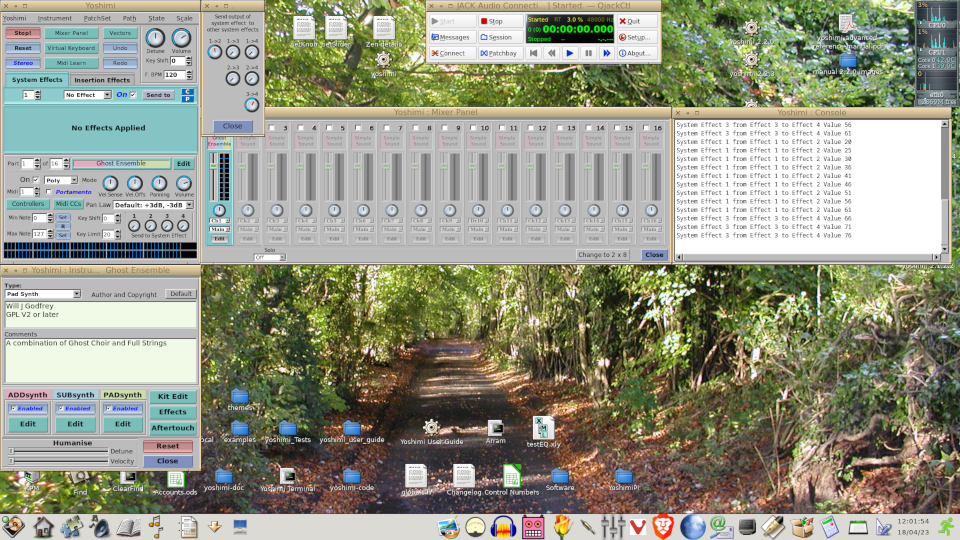
\includegraphics[scale=0.625]{2.2.0/gui_normal.png}
      \caption{Windows at default size}
      \label{fig:default_size_windows}
   \end{figure}

   Next see the same view, but with the Sys Sends window resized to the
   full height of the display. Every item, knobs and labels,
   remains perfectly in scale.

   \begin{figure}[H]
      \centering
      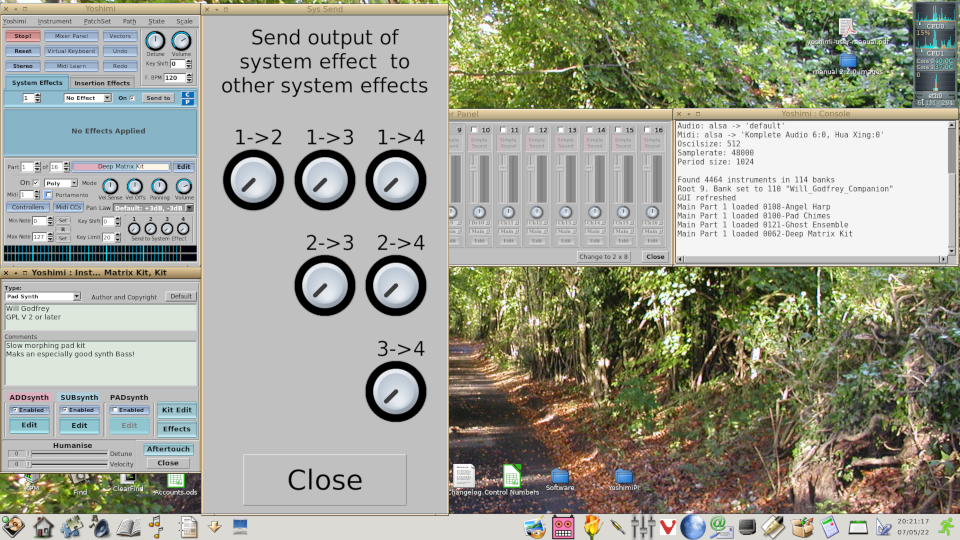
\includegraphics[scale=0.625]{2.2.0/gui_big.png}
      \caption{System Sends window resized}
      \label{fig:resized_sends_window}
   \end{figure}

\subsection{Revised Graphical Interface / The Filer}
\label{subsec:interface_filer}

   One feature that proved impossible to work around was the default FLTK file
   chooser. The only recourse was to replace it with a \textsl{Yoshimi}
   chooser.
   This provided the opportunity to discard all generic features and controls,
   and provide exactly what \textsl{Yoshimi} needed, fitting neatly with
   \textsl{Yoshimi's} uncluttered ethos of only showing what one needs to see.

   Below is a typical entry for loading a patchset.

   \begin{figure}[H]
      \centering
      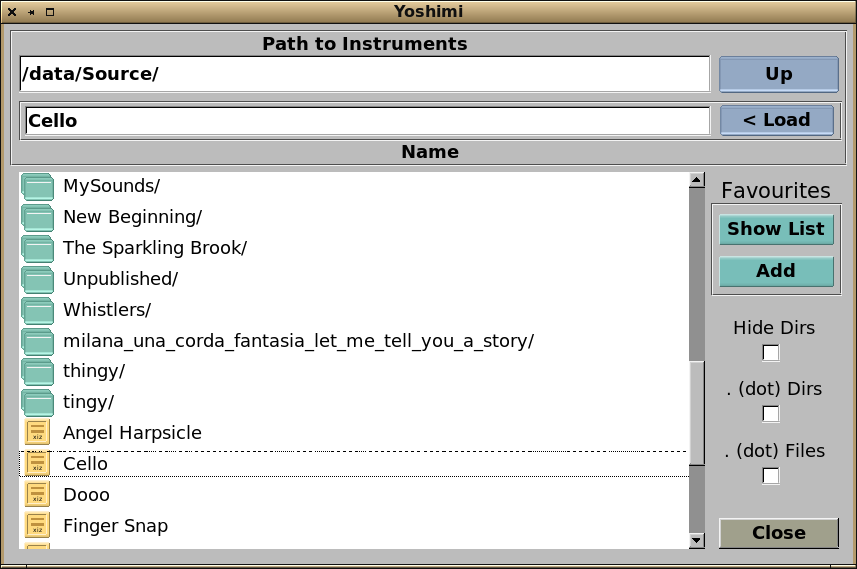
\includegraphics[scale=0.5]{2.1.0/filer.png}
      \caption{A Filer 'Load' Window}
      \label{fig:filer_load_window}
   \end{figure}

   At the top is the \textsl{path} field. One can manually edit this field to go
   to a known route, and on hitting 'Return' the list below it will be updated.
   If saving or exporting files, new directories can added here. A request for
   confirmation will pop up. However it wouldn't make sense to try to load or
   import something from a directory that doesn't yet exist, so this will
   generate an error message.

   The \textsl{Up} button moves back along the directory tree, or one can simply
   edit out one or more directory names and hit 'Return'.

   The \textsl{Load} button simply performs that action on the entry in the
   \textsl{name} field if it is valid. For saving, one can create a
   new name here.

    \textbf{Note:} The Path and Name fields, and the Up and Load buttons,
    change depending on what type of file is being managed. See the examples
    below.

   The main list area shows first the sub-directories found; a double-click
   on these will add them to the path field and re-scan for contents. Below
   these are the files that \textsl{Yoshimi} recognises. A single-click on
   one of these will will place it in the name field where it can be edited,
   whereas a double-click performs the appropriate load/save operation.

   To the side are a number of extra buttons and switches:

   \textsl{Show List} is described below.

   \textsl{Add} places the current path in the favourites list and switches to
   this view for further management.

   \textsl{Hide Dirs} is useful when one knows they have the right path, but the
   directory contains a long list of sub-directories.

   \textsl{.(dot) Dirs} makes these directories visible, although it would be most
   unusual to have these containing valid \textsl{Yoshimi} files.

   \textsl{.(dot) Files} makes these \textsl{Yoshimi} files visible.

   Here are just the headings for several other file types.

   \begin{figure}[H]
      \centering
      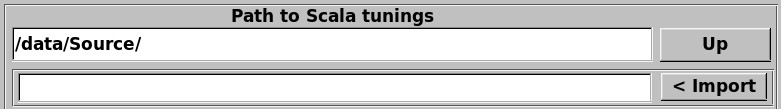
\includegraphics[scale=0.5]{2.1.0/tuning_import.png}
      \caption{A Scala 'import' Window}
   %   \label{fig:filer_scala_window}
   \end{figure}

   \begin{figure}[H]
      \centering
      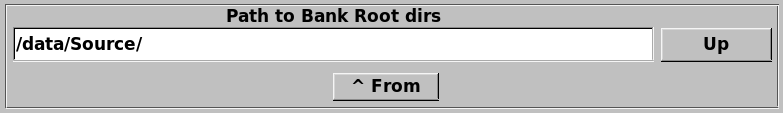
\includegraphics[scale=0.5]{2.1.0/bank_root.png}
      \caption{A Bank 'root' Window}
      \label{fig:filer_bank_root_window}
   \end{figure}

   \begin{figure}[H]
      \centering
      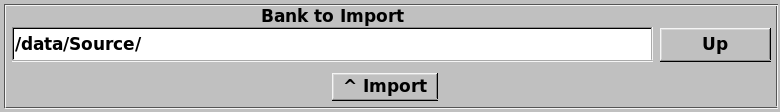
\includegraphics[scale=0.5]{2.1.0/bank_import.png}
      \caption{A Bank 'import' Window}
      \label{fig:filer_bank_import_window}
   \end{figure}

   Neither the bank root nor bank import views have a 'name' field. This is
   because one is directly importing or registering a path containing these
   elements, not the elements themselves. Therefore the path 'leaf' \textbf{is}
   the name. However, when exporting these you will want to give them a name, so
   the field is then present.

% Might need to clarify the paragraph above.

   When selecting 'Show Favourites', the existing filer window
   is overlaid with the
   following view. Notice, it retains the path as a reminder.

   \begin{figure}[H]
      \centering
      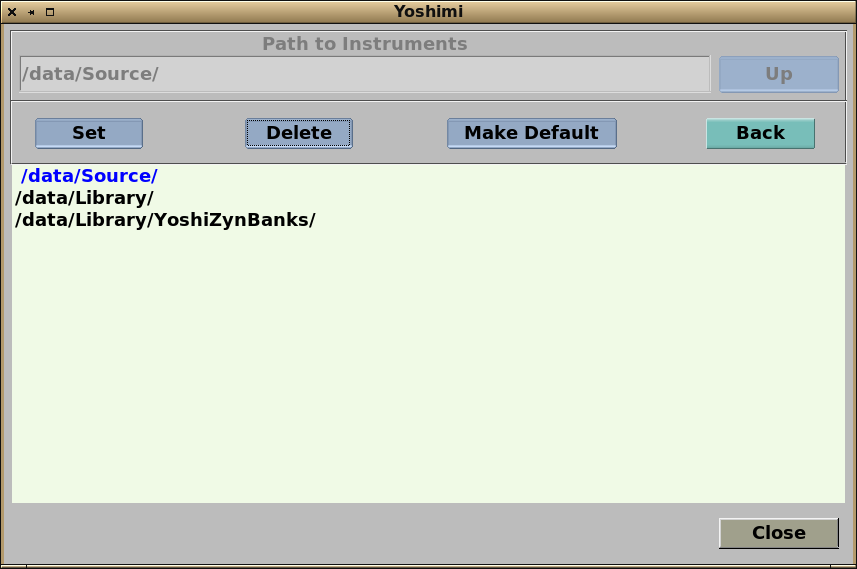
\includegraphics[scale=0.47]{2.2.0/favourites.png}
      \caption{The Filer 'Favourites' Window}
      \label{fig:filer_favourites_window}
   \end{figure}

   A double-click on a path in the filer favourites view will now select it and
   return you to the main filer window.

%-------------------------------------------------------------------------------
% vim: ts=3 sw=3 et ft=tex
%-------------------------------------------------------------------------------
